\documentclass[a4paper]{article}
\usepackage{fullpage}
\usepackage{amsmath}
\usepackage{amssymb}
\usepackage{graphicx}
\usepackage{physics}
%\usepackage[round]{natbib}
%\usepackage{bibtex}
\usepackage{fancyvrb}
\usepackage{hyperref}
\usepackage[linesnumbered,boxed]{algorithm2e}
\usepackage{subfigure}
\usepackage{xcolor}

\numberwithin{equation}{section} % Remove this line for global equation numbering

\title{MATH1058 coursework [40 marks]}
\author{Stefano Coniglio}
\date{\today}

\begin{document}

% This produces the title: to modify contents, change the \title, \author, and
% \date in the preamble
\maketitle




\section{Implementation}

\subsection{[5 marks] Pseudocode for the $O(n^3)$ version}

\textcolor{blue}{
  Report the pseudocode of your implementation "{\tt dijkstra1}".
}


Example (this code is entirely unrelated to the assignment!)

\begin{Verbatim}[numbers=left]
  def dummy_function(myList):
    n = len(myList)
    for i in range(0,n):
      myList[i] = myList[i] + 1
      myList[i] = myList[i] % 2
      for j in range(0,i):
        myList[j] = myList[i] + i
  return myList
\end{Verbatim}
  
%WRITE HERE


\subsection{[5 marks] Show that your implementation indeed has complexity $O(n^3)$}

\textcolor{blue}{
  Proceed as we did in the lectures, analyzing the complexity of each line/block of lines.
}

Example adopting the previous code.

\begin{itemize}
  \item Lines 2 and 5 take $O(1)$.
  %
  \item Each time the block of lines 4-to-7 is repeated:
  %
  \begin{itemize}
    \item Lines 4-to-5  $O(1)$.
    \item Each time it is repeated, line 7 takes O$O(1)$. Since, due to line 6, it is repeated $O(n)$ times, it overall takes $O(n)$.
  \end{itemize}
  %
  Overall, lines 4-to-7 take $O(n)$.
\end{itemize}

Overall, we have a complexity of:
$$
  O(1) + + O(n) \big( O(1) + O(n)\big) = O(n^2).
$$

\subsection{[5 marks] Pseudocode for the $O(n^2)$ version}

\textcolor{blue}{
  Report the pseudocode of your implementation "{\tt dijkstra2}".
}

Example (this code is entirely unrelated to the assignment!)

\begin{Verbatim}[numbers=left]
  def dummy_function(myList):
    n = len(myList)
    for i in range(0,n):
      myList[i] = myList[i] + 1
      myList[i] = myList[i] % 2
      for j in range(0,i):
        myList[j] = myList[i] + i
  return myList
\end{Verbatim}
  
%WRITE HERE


\subsection{[5 marks] Show that your implementation indeed has complexity $O(n^2)$}

\textcolor{blue}{
  Proceed as we did in the lectures, analyzing the complexity of each line/block of lines.
}

Example adopting the previous code.

\begin{itemize}
  \item Lines 2 and 5 take $O(1)$.
  %
  \item Each time the block of lines 4-to-7 is repeated:
  %
  \begin{itemize}
    \item Lines 4-to-5  $O(1)$.
    \item Each time it is repeated, line 7 takes O$O(1)$. Since, due to line 6, it is repeated $O(n)$ times, it overall takes $O(n)$.
  \end{itemize}
  %
  Overall, lines 4-to-7 take $O(n)$.
\end{itemize}

Overall, we have a complexity of:
$$
  O(1) + + O(n) \big( O(1) + O(n)\big) = O(n^2).
$$

%WRITE HERE

\section{Experimental results and analysis}

\subsection{[5 marks] Empirical computing times}

\textcolor{blue}{
  Report the empirical computing times you have computed in Excel for {\tt dijkstra1} and {\tt dijkstra2} ($y_1$ and $y_2$) in a table.
  %
  Report in an Excel line chart the values of $y_1$ versus $n$ and $y_2$ versus $n$.
}

\begin{table}[h!]
  \caption{A table (not related to the coursework). Notice that captions should precede tables, whereas they should follow figures.}
  \begin{center}
\begin{tabular}{l|lll}
  header    & header2 & header3 \\
  \hline
  name1     & 12      & 12\\
  $s = |S|$ & 5       & 42
\end{tabular}
  \end{center}
\label{tab:1}
\end{table}


\begin{figure}[h!]
  \begin{center}
    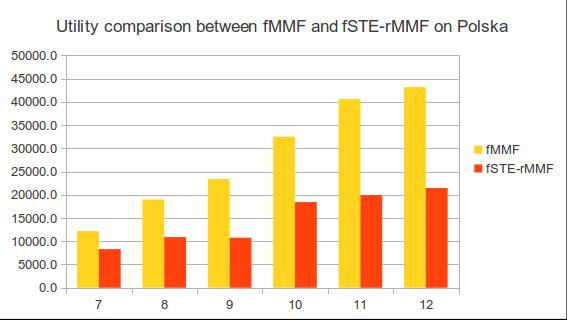
\includegraphics[scale=0.5]{./dummy.png}
  \end{center}
  \caption{A dummy figure (also unrelated to the coursework).}
  \label{fig:a_figure}
\end{figure}

\subsection{[5 marks] Logarithms of the computing times}

\textcolor{blue}{
  Report the logarithms of the empirical computing times you have computed in Excel for {\tt dijkstra1} and {\tt dijkstra2} ($\log(y_1)$ and $\log(y_2)$) in a table.
  %
  Report in an Excel line chart the values of $\log(y_1)$ versus $\log(n)$ and $\log(y_2)$ versus $\log(n)$.
}

\begin{table}[h!]
  \caption{Another dummy table.}
  \begin{center}
\begin{tabular}{l|lll}
  header    & header2 & header3 \\
  \hline
  name1     & 12      & 12\\
  $s = |S|$ & 5       & 42
\end{tabular}
  \end{center}
\label{tab:1}
\end{table}


\begin{figure}[h!]
  \begin{center}
    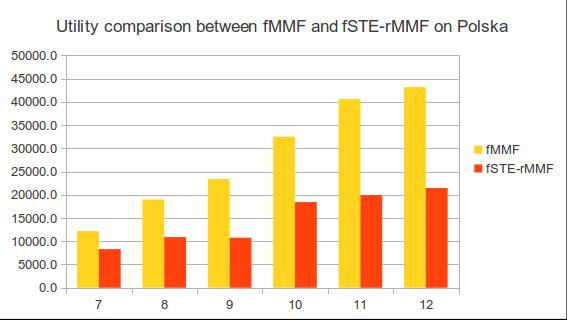
\includegraphics[scale=0.5]{./dummy.png}
  \end{center}
  \caption{Another dummy figure.}
  \label{fig:a_figure}
\end{figure}




\subsection{[5 marks] Estimated complexities}

\textcolor{blue}{
  Report the computational complexities of {\tt dijkstra1} and {\tt dijkstra2} ($y'_1$ and $y'_2$) you have estimated in Excel via linear/affine regression as two functions of $n$.
}

%WRITE HERE, OVERWRITING THE EXAMPLE

Example using dummy functions:
%
\begin{equation}\label{eq:1}
  y'_1 = \sin(n)
\end{equation}

\begin{equation}\label{eq:2}
  y'_2 = \tan(n)
\end{equation}


\subsection{[5 marks] Speedup}

\textcolor{blue}{
  Report the estimated speedup {\tt dijkstra2} w.r.t. {\tt dijkstra1} as the function (of the instance size $n$) $\frac{y'_2}{y'_1}$.
  %
  Compare this empirical speedup to the theoretical one (the latter is equal to the ratio of the computational complexities of your implementations, expressed in big-O notation.
  %
  Is the empirical one smaller or larger than the theoretical one? Motivate the answer.
}

%WRITE HERE, OVERWRITING THE EXAMPLE

Example using dummy functions:
%
\begin{equation}
  \frac{y'_2}{y'_1} = \frac{\sin(x)}{\tan(n)}
\end{equation}

Theoretical speedup:
\begin{equation}
  \frac{O(n^8)}{O(n^{11})} = O(n^{-2}).
\end{equation}



Some explanation should be written here.

\end{document}
